
\section{Numerical Investigations of Antennas in TEM Cells}

\subsection{Preliminary Considerations for Numerical Analysis}

\subsubsection{Skin Effect}

The Skin-effect causes current to flow through a reduced area in a conductor, thus increasing resistance. The imaginary part $\kappa$ of the complex wave number $k$ is described by

\begin{equation}
	\kappa = \omega \sqrt{\frac{\epsilon \mu}{2}}\left[\sqrt{ 1+\left(\frac{\sigma}{\epsilon\omega}\right) ^2 } -1\right]^{1/2}.
	\label{eqn:kappa}
\end{equation}

The skin depth $d$ is responsible for the increased conductor losses and is expressed as 

\begin{equation}
	d = 1/\kappa.
	\label{eqn:skin_depth}
\end{equation}

For highly conductive materials $\left(\sigma \ll \epsilon\omega\right)$ the skin depth is $d \propto 1/\sqrt{\omega}$. Conductor losses $P_\mathrm{loss}$ are linearly proportional to the area of the conductor and therefore Skin-depth. They show the same dependency on the frequency $P_\mathrm{loss}\propto 1/\sqrt{\omega}$ \cite[p. 413]{Griffiths_2024}. Conductor losses contribute to the power consumption of the small loop antenna and is significantly larger than radiation power \cite[p. 231]{Balanis_1997}. 

The investigations in this thesis focus on the coupling behavior of antennas, including the radiation power consumed. All conducting surfaces in the simulation models are perfect electric conductors (PEC) to remove the impact of the Skin-effect.

%reduces the area in which the current flows, therefore increasing resistance. This appears due to the reduction of the depth, in which the electromagnetic waves enter. It is also called Skin depth and mathematically described by \autoref{eqn:skin_depth}. It depends on the imaginary part of the wave number $\kappa$, which is described in \autoref{eqn:kappa}. For high conducting materials $\left(\sigma >> \epsilon\omega\right)$, the dependency of the skin depth $d$ on the frequency can be described therefore as $d \propto 1/\sqrt{\omega}$. Since the power dispersion is linearly proportional to the area of the conductor and therefore Skin-depth, it shows the same dependency on the frequency $P_\mathrm{disp}\propto 1/\sqrt{\omega}$ \cite{Griffiths_2024}.  
%\todo{Own little chapter for skin effect? Loop antennas are known for higher conductor losses than radiation Balanis page 231}
%
%\begin{subequations}
%	\begin{equation}
%		\kappa = \omega \sqrt{\frac{\epsilon \mu}{2}}\left[\sqrt{ 1+\left(\frac{\sigma}{\epsilon\omega}\right) ^2 } -1\right]^{1/2}
%		\label{eqn:kappa}
%	\end{equation}
%	\begin{equation}
%		d = 1/\kappa
%		\label{eqn:skin_depth}
%	\end{equation}
%\end{subequations}
%
%\autoref{fig:deleteafter} shows the total power maintained in the system, meaning $S_{11}^2+S_{12}^2+S_{13}^2$. It does not add up to one, meaning that some energy is lost due to finite conductivity of the septum and antenna. This energy dispersion increases with frequency, most likely due to a decrease of the conductivity due to high-frequency effects like the Skin-effect. Consequently, the power consumption in \autoref{fig:currentlooppowerconsumption} shows a square root relation to the frequency, because the power dispersion is so high. When changing the material of the antenna and septum to a perfect electric conductor, the total power in a system remains one (no power is dispersed) and the power consumption over frequency of the antenna shows a quadratic relation to the frequency, due to the quadratic increase of the radiation resistance.
%
%
%
%At 1\,GHz, the dispersed power already equals to 0.46\,\%, which is much higher than the power transfer of the antenna to one waveport of 1.26e-5 at that frequency. Because this dispersed power is proportional to the square-root of the frequency $P_\mathrm{disp}\propto 1/\sqrt{\omega}$, the overall transferred power to the antenna shows the same characteristic. However, the power transfer to the waveports has a quadratic dependency on the frequency. %This, in turn, also leads to the unusual relation of the electric dipole moment to the frequency. 
%
%This dispersed power may be ignored in the simulations by changing the antenna's material (main source of power dissipation) and the septum from copper to a perfect electric conductor. The overall power in the system then remains at a constant one over the whole frequency range. Additionally, the transferred power to the antenna now has a quadratic relationship with the frequency, indicating increased radiation efficiency, previously described by \autoref{eqn:elec_rad_res}. 
%\todo{Show plots?}

\subsubsection{Antenna models}\label{sec:antenna_model}

Every antenna is fed with a round feedpoint, shown in \autoref{fig:antennaport}. They provide an incident wave of unit power (1\,W). The antenna wires are modeled as PECs with a diameter of 0.2\,mm. The geometry is intentionally kept simple, with the cylindrical wires pointing either in x-, y- or z-direction, without combining multiple orientations. 

\begin{figure}[h]
	\centering
	\includegraphics[width=0.7\linewidth]{content/img/antenna_port}
	\caption{Geometry of an antenna's feedpoint used in simulation. The antenna is fed through a round waveport of diameter $0.46\,\mathrm{mm}$. The antenna consists of PEC wire with diameter of $0.2\,\mathrm{mm}$.	This geometry leads to a reference impedance of $Z_0\approx 50$\,$\Omega$.}
	\label{fig:antennaport}
\end{figure}




\subsubsection{TEM cell model}

The TEM cell model used has a width of $a=40$\,mm, a height of $b=24$\,mm and a length of $l=100$\,mm, shown in \autoref{fig:tem_cell_model}. The cell walls and septum are modeled as PECs. In the TEM cell simulation model, the tapered transition sections at the ports are omitted. This simplification allows unrestricted propagation of higher-order modes, facilitating investigations of their coupling behavior with antennas. \todo{reference section where I discussed this} The reference impedances of the output ports equal $Z_0 \approx 50\,\Omega$.

\begin{figure}[htbp]
	\centering
	\begin{subfigure}[b]{0.48\textwidth}
	\centering
\includegraphics[width=1\linewidth]{content/img/tem_cell_front}
\caption{xy-plane}
\label{fig:temcellfront}
	\end{subfigure}
	\hfill
	\begin{subfigure}[b]{0.48\textwidth}
	\centering
\includegraphics[width=1\linewidth]{content/img/tem_cell_side}
\caption{yz-plane}
\label{fig:temcellside}
	\end{subfigure}
	
	\caption{Geometrical arrangement of the TEM cell used in simulations. The front shows the xy-plane, and the side the yz-plane of the TEM cell.}
	\label{fig:tem_cell_model}
\end{figure}

Upon exciting the output ports, the electric and magnetic energy $W_\mathrm{e}$ and $W_\mathrm{m}$ stored in the TEM cell is derived by \autoref{eqn:em_energy}. The current and voltage at the output ports is found with \crefrange{eqn:iin}{eqn:vin}. The capacitance and inductance of the TEM cell are given by \crefrange{eqn:l_m_energy}{eqn:c_e_energy}. The reactance values fluctuate negligibly over frequency likely due to numerical inaccuracies. The average capacitance and inductance values over the frequency range are chosen. It is assumed that the TEM cell has a constant capacitance and inductance of $C_\mathrm{T} = 6.74\,\mathrm{pF}$ and $L_\mathrm{T} = 16.25\,\mathrm{nH}$. 

\subsubsection{Dipole moments models}\label{sec:prep_dip}

A magnetic dipole moment can be expressed equivalently as either an electric current $I_0$ in a loop, or a magnetic current $I_\mathrm{m}$ in a line, as described in \autoref{eqn:magn_current_curr_loop}. All dipole moments used in the simulations are assumed to be of infinitesimal length, as discussed in \autoref{sec:infinitesimal_electric_dipoles} and \autoref{sec:mag_dip}. For infinitesimal magnetic dipoles, \autoref{eqn:magn_current_curr_loop} simplifies to 

\begin{equation}
	|\mathbf{m}_{\mathrm{m}}|=j\omega\mu_0 |\mathbf{m}_{\mathrm{0}}|,
	\label{eqn:m_mymag_ifa}
\end{equation}

where $\mathbf{m}_{\mathrm{m}}$ with the unit Vm denotes the magnetic dipole moment in the magnetic current representation, and $\mathbf{m}_{\mathrm{0}}$ with the unit Am$^2$ the moment in the electric current representation \cite{10742020}. The simulation models represent magnetic dipole moments with $\mathbf{m}_{\mathrm{m}}$, which will be used in further investigations.

The electric and magnetic dipole moments are placed at the center of the TEM cell at $x=0$, $y=b/2$, $z=0$. As discussed in \autoref{sec:field_dist}, $\mathbf{e}^\pm_\mathrm{TEM}(x=0, y=b/2, z=0)$ has only a y-component at this location, while $\mathbf{h}_\mathrm{TEM}^\pm(x=0, y=b/2, z=0)$ has only an x-component. Consequently, the equivalent dipole moment $\mathbf{m}_{\mathrm{e}}$ is oriented along the y-direction, and $\mathbf{m}_{\mathrm{m}}$ along the x-direction.

Placing $\mathbf{m}_{\mathrm{m}}$ and $\mathbf{m}_{\mathrm{e}}$ in the center of the TEM cell therefore significantly simplifies modeling electrically small antennas with equivalent dipole moments. This assumption is valid for the TEM mode. This configuration is assumed for all numerical investigations following in this thesis, unless otherwise stated.

 When normalizing to the free-space wave impedance $Z_0$, $\mathbf{m}_\mathrm{e}$ can be interchanged with an equivalent $\mathbf{m}_\mathrm{m}$ and vice-versa \cite[p. 414]{Jackson}. Therefore, normalizing either $\mathbf{m}_{\mathrm{e}}$ or $\mathbf{m}_{\mathrm{m}}$ to the free-space wave impedance $Z_0$ enables a meaningful comparison between them.

All simulation results are counterchecked by inserting the equivalent dipole moments into the TEM cell and comparing the power and phase at the output ports with the antenna's results.

\autoref{fig:eyezcouplingcomparison} demonstrates the normalized output power of an electric dipole moment pointing in y-direction, and one in z-direction. This simulation only demonstrates the coupling behavior of the dipole moments over frequency, to explain the non-linear coupling of certain antennas. If dipole moments in certain positions and orientations couple with a different proportionality than the standard two dipole moments (ez and my), then the non-linear coupling may be explained that way.

\begin{figure}[h]
	\centering
	\includegraphics[width=0.5\linewidth]{content/img/ey_ez_coupling_comparison}
	\caption{Comparison of normalized output power of electric dipole moments}
	\label{fig:eyezcouplingcomparison}
\end{figure}



The electric dipole moment in z-direction $e_\mathrm{z}$ demonstrates the expected behavior: As the frequency rises, this dipole moment rises linearly and thus increases the output power quadratically. The electric dipole moment in y-direction $e_\mathrm{y}$ also increases linearly increase with frequency, but does not significantly change the output power for the low frequencies. However, as the frequency approaches the cut-off frequency of the next-higher order mode, the coupling rises significantly.

This simulation is repeated where the dipole moments are located at a height of $h=6\,\mathrm{mm}$, which is the dead center of the TEM cell, and $h=9\,\mathrm{mm}$, which is near the top wall of the TEM cell. The simulation results are similar for both cases. 

Most importantly, this simulation shows that the dipole moments have a relation to the frequency independent on their position. While their magnitude themselves do depend on the position, the relation to the frequency does not. 

An electric dipole in direction of propagation lead to no power transfer, even in higher order modes. That's because these fields do not overlap with the dipole, for which TM modes would be necessary.

\todo{Repeat Simulation for several other dipole moment positions and orientations?} 

As show in the previous simulations, antennas may be represented by dipole moments. This can be done in simulation models, which would otherwise be computationally too effortful. The dipole moments may be put into a shielded enclosure around a larger electronic system, as has been done in \cite{10274360}.

\subsubsection{Mesh modifications}\label{sec:mesh}

The mesh determines the resolution of the field quantities over the computational domain. Since electrically small conductors are involved, implementing small mesh elements in their proximity is necessary for accurate modeling of near-fields. Adaptive meshing algorithms may neglect this task, due to the low impact of these near-fields on the solution of the overall computational domain. Consequently, adjusting mesh element sizes does not significantly influence the overall solution of the model, but greatly improves the accuracy of near-field investigations.

The maximum mesh element length in error-prone volumes are adjusted, until the obtained results show a reasonably low amount of numerical artifacts. Such volumes are commonly located adjacent to feedpoints and along edges of small conductors, where large field intensities occur within small spatial regions. The simulation models used in this thesis use roughly 15 elements on the surfaces of such critical volumes to achieve a reasonable representation of these regions while avoiding excessively large meshes.

\subsubsection{S-parameters and derived data}\label{sec:s-param-data}

The TEM cell with an antenna is modeled as a three-port network. The two output ports of the TEM cell are denoted as ports 1 and 2, while the antenna feedpoint is marked as port A. The behavior of this system is fully characterized by its scattering matrix, given as

\begin{equation}
	\left[S\right]=
	\begin{bmatrix}
		S_{11} & S_{12} & S_{1A} \\
		S_{21} & S_{22} & S_{2A} \\
		S_{A1} & S_{A2} & S_{AA}
	\end{bmatrix}.
\end{equation}

The coupling between the antenna and the two ports of the TEM cell are described by S-parameters, specifically the forward transmission coefficients $S_{\mathrm{A1}}$ and $S_{\mathrm{A2}}$. The phases of the forward transmission coefficients $\Phi_\mathrm{A1}$ and $\Phi_\mathrm{A2}$ provide information on the phase shift between the incident wave at port A, and the transmitted wave at output ports 1 and 2. The magnitude of this coefficient is the same for the antenna to both ports $|S_{\mathrm{A1}}|=|S_{\mathrm{A2}}|$, given that the antenna is placed far from the output ports. The power transferred from the antenna $P_{\mathrm{A}}$ to the output ports $P_{\mathrm{1}}$ and $P_{\mathrm{2}}$ is derived through
  
  \begin{equation}
  	P_{\mathrm{A}}=\frac{P_{\mathrm{1}}}{10^{|S_{\mathrm{A1}}|/10}}=\frac{P_{\mathrm{2}}}{10^{|S_{\mathrm{A2}}|/10}}.
  	\label{eqn:power_antenna}
  \end{equation}
  
  Consequently, if the normalized electric field distribution of the TEM mode $\mathbf{e^\pm}_\mathrm{TEM}$ is unknown, it may be derived by setting the output power of a waveport to $P_{\mathrm{1}}=P_{\mathrm{2}}=1/2\,\mathrm{W}$. For example, the uniformly distributed, normalized electric field of the TEM mode along the y-axis at the center of the TEM cell ($z=0$, $x=0$) is derived by
  
  \begin{equation}
  	|a_\mathrm{TEM}|\cdot\mathbf{e}_\mathrm{TEM}^+(x=0,y,z=0)= \frac{\sqrt{P_\mathrm{1}Z_\mathrm{0}}}{b/2}.
  \end{equation}
  
  The difference in phase of $S_{\mathrm{A1}}$ and $S_{\mathrm{A2}}$ influences the magnitude of magnetic dipole moments and electric dipole moments, as discussed in \autoref{sec:equ-dip-mom}. 
%  In this case, a phase shift of $\pi$ indicates the presence of a magnetic dipole moment and the absence of electric dipole moments. This is shown by
%  
%  \begin{subequations}
%  	\begin{equation}
%  		\mathbf{m}_\mathrm{e} = \frac{a+b}{\mathbf{E}^\pm} = \frac{a+a\cdot e^{j\pi}}{\mathbf{E}^\pm} = 0,
%  	\end{equation}
%  	\begin{equation}
%  		\mathbf{m}_\mathrm{m} = j\frac{a-b}{\mathbf{E}^\pm\cdot k_0} = j\frac{a-a\cdot e^{j\pi}}{\mathbf{E}^\pm\cdot k_0} = j\frac{2a}{\mathbf{E}^\pm\cdot k_0}.
%  		\label{eqn:me_phase}
%  	\end{equation}
%  \end{subequations}
%  
%  A phase shift of zero indicates the opposite case. The influence of the electric and magnetic dipole moment is equal, if the phase shift equals $\pi/2$. 
   The peak value of the current through the feedpoint of the antennas is calculated with the S-parameters,
  
  \begin{equation}
  	I_{\mathrm{A}} = \sqrt{2P_{\mathrm{A}}}\frac{(1-S_{\mathrm{AA}})}{\sqrt{Z_0}}.
  	\label{eqn:iin}
  \end{equation}
  
  $P_{\mathrm{A}}$ is the incident power wave applied to the port. 
  The peak voltage at the feedpoint is calculated in a similar fashion as 
 
 \begin{equation}
 	V_{\mathrm{A}} = \sqrt{2P_{\mathrm{A}}}(1-S_{\mathrm{AA}})\sqrt{Z_0}.
 	\label{eqn:vin}
 \end{equation}
 
 Another method to derive voltages and currents is by integration of field intensities. Special care has to be taken at mesh refinement in the area of integration to reduce numerical errors. 
 
 The impedance seen from the antenna feedpoint is 
 
 \begin{equation}
 	Z_{\mathrm{A}}=Z_0\frac{1+S_{\mathrm{AA}}}{1-S_{\mathrm{AA}}}.
 	\label{eqn:za}
 \end{equation}
 
 All values are peak values, unless otherwise stated. 
 
 \subsubsection{Investigation of field regions}
 
\todo[inline]{Update field plots}
 
In this section, the coupling-field regions described in \autoref{sec:rad_fields} are analyzed using the model shown in \autoref{fig:krtemcell}. This analysis examines whether frequency-dependent coupling behavior of the TEM cell can be attributed to changes in the dominant coupling-field region.

 \begin{figure}[h]
 	\centering
 	\includegraphics[width=0.7\linewidth]{content/img/kr_tem_cell}
 	\caption{A TEM cell containing an electric $\mathbf{m}_\mathrm{e}$ and a magnetic dipole moment $\mathbf{m}_\mathrm{m}$ in the center $x=0, y=r=b/4, z=0$ to investigate the field regions in which the coupling occurs.}
 	\label{fig:krtemcell}
 \end{figure} 
 
To determine the influence of the field regions on the coupling effect, $\mathbf{m}_\mathrm{e}$ and  $\mathbf{m}_\mathrm{m}$ are placed in two different TEM cells of dimensions  $a=10\,\mathrm{mm}, b=6\,\mathrm{mm}$ and $a=40\,\mathrm{mm}, b=24\,\mathrm{mm}$. The $k\cdot r$-factor for both cases is shown in \autoref{fig:kranalysissmalltem}.

 \begin{figure}[htbp]
	\centering
	\centering
	\includegraphics[width=0.5\linewidth]{content/img/kr_analysis_small_TEM}
	\caption{$k\cdot r$ in small TEM cell}
	\label{fig:kranalysissmalltem}
	\hfill
\end{figure}

aking the TEM cell smaller such that $k\cdot r \ll 1$, proves to be feasible. The following simulations are conducted with a TEM cell of dimensions $a=10\,\mathrm{mm}$ and $b=6\,\mathrm{mm}$, visible in \autoref{fig:krtemcell}.  
 
 
 First, the current loop antenna used in \autoref{sec:loop_sim} is placed in the dead center of the TEM cell. The equivalent dipole moments are shown in \autoref{fig:loop_small_tem_moments}. In the \autoref{fig:dipole_moments_loop_antenna_copy} next to it, the dipole moments of the same antenna in the larger TEM cell used before ($a=40\,\mathrm{mm}$ and $b=24\,\mathrm{mm}$) are presented. 
 
 \todo[inline]{TODO:Redo plots}
 
 \begin{figure}[htbp]
 	\centering
 	\begin{minipage}[t]{0.48\textwidth}
 		\centering
 		\includegraphics[width=1\linewidth]{content/img/loop_small_tem_moments.png}
 		\caption{Moments in small TEM cell}
 		\label{fig:loop_small_tem_moments}
 	\end{minipage}
 	\hfill
 	\begin{minipage}[t]{0.48\textwidth}
 		\centering
 		\includegraphics[width=1\linewidth]{content/img/dipole_moments_loop_antenna.png}
 		\caption{Moments in normal TEM cell}
 		\label{fig:dipole_moments_loop_antenna_copy}
 	\end{minipage}
 \end{figure}
 
 This is done to compare the dipole moments in both cases. While they clearly increased by magnitude in case of the small TEM cell due to better coupling, their non-linear frequency relation still remains. This means that the change of field regions is not the reason for this behavior.
 
 \todo{TODO: Insert kr, describe where r is measured, describe why the suspicion was that kr could influence this and how the fields change in the regions as described in the theoretical parts. Insert small current loop simulation. Insert Dipole Moment Simulations}
 
 The $k\cdot r$ factor is determined in \autoref{fig:kranalysissmalltem} in the frequency range from 1\,MHz to 3\,GHz for the small TEM cell. This factor does not surpass 0.1, thus fulfilling the requirement $k\cdot r \ll 1$ for this investigation. For comparison, the $k\cdot r$ factor over a wider frequency range are shown in \autoref{fig:kranalysissmalltem} for the normal sized TEM cell ($a = 40\,\mathrm{mm}$ and $b = 24\,\mathrm{mm}$) and a degenerately high TEM cell ($a = 10\,\mathrm{mm}$ and $b=44\,\mathrm{mm}$). The high TEM does not have a port impedance of $50\,\Omega$, and is an attempt to achieve a large $k\cdot r$ factor without higher-order modes propagating. The markers in \autoref{fig:kranalysis} indicate the cut-off frequency, in which the next higher-order mode propagates. They demonstrate, that even in the high TEM cell a $k\cdot r = 1$ is not achieved.
 
 

 \todo[inline]{Fix figures: Titles and Legends. Add kr of normal cell.}
 
% \begin{minipage}[t]{0.48\textwidth}
% 	\centering
% 	\includegraphics[width=1\linewidth]{content/img/kr_analysis}
% 	\caption{$k\cdot r$ for other TEM cells}
% 	\label{fig:kranalysis}
% \end{minipage}
 
 Now, three simulations are conducted with different excitation sources in the small TEM cell:
 
 \begin{itemize}
 	\item The current loop 
 	\item The equivalent dipole sources $e_z$ and $m_m$ of the current loop
 	\item The equivalent magnetic dipole source $m_m$, neglecting $e_z$
 \end{itemize}
 
 \autoref{fig:outputpowercomparisonsmalltem} shows the output power over frequency normalized to 1\,W for all three constellations. The normalization is done to qualitatively discuss the frequency-dependent coupling behavior. \autoref{fig:phaseshiftcomparisonsmalltem} demonstrates the phase shift between the powers at the two waveports over frequency.
 
 \begin{figure}[htbp]
 	\centering
 	\begin{minipage}[t]{0.48\textwidth}
 		\centering
 		\includegraphics[width=1\linewidth]{content/img/output_power_comparison_small_tem}
 		\caption{Output powers}
 		\label{fig:outputpowercomparisonsmalltem}
 	\end{minipage}
 	\hfill
 	\begin{minipage}[t]{0.48\textwidth}
 		\centering
 		\includegraphics[width=1\linewidth]{content/img/phase_shift_comparison_small_tem}
 		\caption{Phase shifts}
 		\label{fig:phaseshiftcomparisonsmalltem}
 	\end{minipage}
 \end{figure}
 
 The frequency dependent behavior of the output power does not change depending on the type of dipole moment used. This is significant, because this shows that the dipole moments do not exhibit different coupling behaviors in the TEM cells. This is further proven in the phase shift plots. The magnetic dipole moment causes a constant phase shift of $-\pi$. If this was not the case, this would mean that the coupling behavior of the magnetic dipole moment in the TEM cell would change. Since the opposite is the case, this poses as good evidence against arguments of change in field regions causing the non-linear dipole moment behavior. Instead, it is very likely to be caused by the geometry of the antenna.

\FloatBarrier

